\documentclass{standalone}
    \usepackage{amsmath}
    \usepackage{amsthm}
    \usepackage{amssymb}
    
    \usepackage{tikz}
    \usepackage{standalone}
    \usetikzlibrary{calc}
    \usepackage{pgfplots}
    \usepackage{color}
    
    \begin{document}
    
        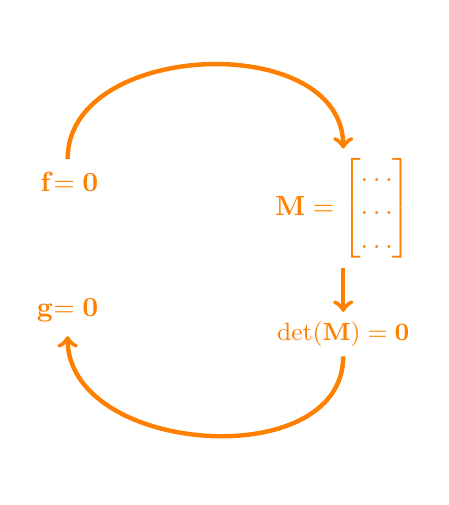
\begin{tikzpicture}
    
        \node (0) at (-0.5, 0.3) {\textcolor{orange}{$\begin{aligned}
            \mathbf{f} & \mathbf{= 0 }\\
            & \\
            & \\
            \mathbf{g} & \mathbf{= 0 }\\
             \end{aligned}$}};

        \node(1) at (3, .8) {\textcolor{orange}{$\mathbf{M} = \begin{bmatrix}
            \dots \\
            \dots \\
            \dots
          \end{bmatrix}$}};
        \draw (0) edge[out=90, in=90, ->, ultra thick, orange, looseness=1.1] node [above] {} (1);

        \node(2) at (3, -.8) {\textcolor{orange}{\small{det$\mathbf{(M)= 0}$}}};
        \draw (1) edge[out=-90, in=90, ->, ultra thick, orange] node [above] {} (2);
        \draw (2) edge[out=-90, in=-90, ->, ultra thick, orange, looseness=1.1] node [above] {} (0);
        \end{tikzpicture}

    \end{document}